%-----------------------------------------------------------------------------%
\chapter{\babSatu}
%-----------------------------------------------------------------------------%


%-----------------------------------------------------------------------------%
\section{Latar Belakang}
%-----------------------------------------------------------------------------%
Badan Pusat Statistik (BPS) merupakan suatu lembaga pemerintah non-departemen yang bertanggung jawab dalam penyediaan statistik dasar di Indonesia \citep{bps_badan_2016}. Dalam peranannya sebagai penyedia data, BPS melakukan pengumpulan data dengan 2 (dua) metode, yaitu primer dan sekunder. Pengumpulan data primer dilakukan dengan mewawancarai langsung responden, baik responden individu, rumah tangga, maupun perusahaan. Di sisi lain, pengumpulan data sekunder dilakukan dengan mengompilasi data yang telah dikumpulkan oleh pihak lain.


Dalam pengumpulan data primer atau yang biasa disebut dengan pencacahan, suatu wilayah administrasi dibagi menjadi beberapa Blok Sensus (BS) sebagai satuan wilayah kerja pencacahan \citep{bps_sistem_2016}. Setiap petugas pencacahan dapat memiliki beban tugas berupa 1 (satu) atau lebih BS, dimana pada masing-masing BS terdapat rumah tangga yang menjadi target pencacahan. \autoref{fig:capi-ilustration} memberikan ilustrasi pembagian BS dalam desa/kelurahan. 


\begin{figure}[!]
    \centering
    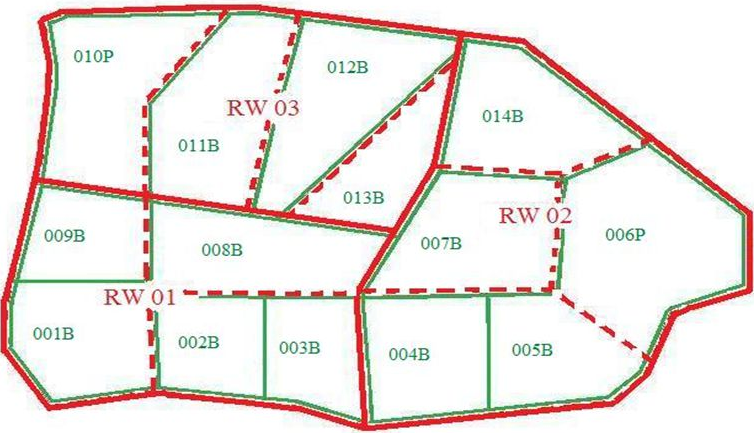
\includegraphics[width=10cm]{Resources/Images/peta_kelurahan_per_bs}
    \caption{Pembagian Blok Sensus dalam Desa/Kelurahan}
    \label{fig:capi-ilustration}
\end{figure}


Alokasi BS kepada masing-masing petugas pencacahan bukanlah suatu perkara yang mudah. \textit{Subject matter} selaku penanggung jawab sensus/survey harus membuat alokasi wilayah kerja yang memenuhi kriteria berikut: 
\begin{enumerate}
	\item Minimum total waktu dan biaya 
	\item Lokasi tugas relatif dekat dengan kantor BPS atau wilayah domisili petugas. 
\end{enumerate}
Alokasi wilayah kerja yang kurang cermat dapat mengakibatkan terjadinya ketimpangan dalam total waktu penyelesaian tugas antar pencacah. Kondisi ini dapat menyebabkan terlambatnya kegiatan pencacahan secara keseluruhan.


Total waktu pencacahan terdiri dari 2 (dua) komponen utama, yakni waktu tempuh antar wilayah kerja dan lama pencacahan dari seluruh wilayah kerja. Lama pencacahan dalam sebuah wilayah kerja meliputi lama perpindahan antar rumah tangga dan lama wawancara pada seluruh rumah tangga di wilayah kerja. Berdasarkan \citep{sudman_time_1965}, komposisi waktu yang dihabiskan oleh seorang pencacah tersusun atas: 21 persen untuk berpindah antar wilayah kerja, 15 persen untuk berpindah antar rumah tangga, 15 persen untuk keseluruhan wawancara, dan sisanya untuk kegiatan lain seperti pengenalan wilayah dan perbaikan data.


Permasalahan alokasi wilayah kerja pencacahan memiliki kesamaan karakteristik \textit{Vehicle Routing Problem} (VRP), atau lebih tepatnya \textit{Multi Depot Vehicle Routing Problem} (MDVRP). VRP merupakan suatu permasalahan yang bertujuan untuk menentukan rute terbaik yang harus ditempuh oleh beberapa kendaraan kurir untuk mengirimkan barang kepada konsumen \citep{dantzig_truck_1959}. Sementara MDVRP adalah varian dari VRP dimana terdapat lebih dari satu depot yang digunakan. Depot merupakan lokasi dimana kendaraan memulai dan mengakhiri perjalanan.


\begin{figure}[!]
    \centering
    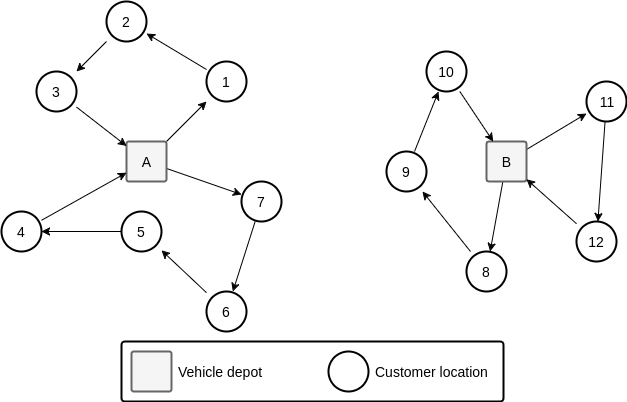
\includegraphics[width=12cm]{Resources/Images/mdvrp-illustration}
    \caption{Ilustrasi \textit{Multi Depot Vehicle Routing Problem}}
    \label{fig:mtsp-ilustration}
\end{figure}


Penyelesaian MDVRP bertujuan untuk mendapatkan solusi dengan total biaya terkecil. Solusi yang dihasilkan berupa sejumlah rute yang terdiri dari sejumlah konsumen yang harus dikunjungi oleh masing-masing kendaraan. Penyelesaian MDVRP harus mengikuti beberapa aturan, yaitu:

\begin{enumerate}
	\item Setiap konsumen hanya dapat dikunjungi sekali dan hanya oleh satu kendaraan. 
	\item Setiap kendaraan memulai dan mengakhiri perjalanan pada sebuah depot yang sama. 
	\item Total \textit{demand} dari seluruh konsumen pada setiap rute tidak melebihi kapasitas dari kendaraan 
\end{enumerate}


Pada permasalahan pembagian wilayah kerja, pencacah dianalogikan sebagai kendaraan, wilayah kerja dimisalkan sebagai konsumen, dan lokasi dimana pencacah memulai perjalanan (rumah atau kantor) dapat diibaratkan sebagai depot.


Pada permasalahan MDVRP terdapat 2 (dua) variabel yang dapat mempengaruhi solusi atau rute yang dihasilkan, yaitu biaya tempuh antar konsumen dan lama pelayanan pada setiap konsumen. Biaya tempuh umumnya didefinisikan dalam satuan waktu sehingga dapat didekati dengan lama tempuh. Kedua variabel ini analog dengan lama tempuh antar wilayah kerja dan lama pencacahan dari setiap wilayah kerja pada permasalahan alokasi wilayah kerja. 


Terdapat beberapa pendekatan yang dapat digunakan untuk mengestimasi lama tempuh antar wilayah kerja, seperti melalui perkiraan, survei, atau menggunakan \textit{service} seperti Google Direction API. Akan tetapi, lama pelayanan pada setiap wilayah kerja tidak dapat diketahui hingga wilayah kerja tersebut selesai dicacah. Hal ini menyebabkan rute-rute yang dihasilkan berpotensi memiliki standar deviasi yang tinggi. \autoref{fig:illustration-timeline-mdvrp} memberikan ilustrasi untuk potensi masalah ini yang dijabarkan sebagai berikut:

\begin{enumerate}
	\item Solusi yang diperoleh dengan menggunakan estimasi lama pelayanan pada setiap wilayah kerja menghasilkan rute terbaik yang relatif \textit{equal} dari segi total waktu (\autoref{fig:illustration-timeline-mdvrp-timeservice-estimation}), 
	\item Setelah semua wilayah kerja dikunjungi, ternyata lama pelayanan pada masing-masing wilayah kerja bervariasi, sehingga variasi total waktu pencacahan menjadi besar (\autoref{fig:illustration-timeline-mdvrp-timeservice-real}).
\end{enumerate}


\begin{figure}[!]
	\centering
	\begin{subfigure}[t]{12.5cm}
		\centering
		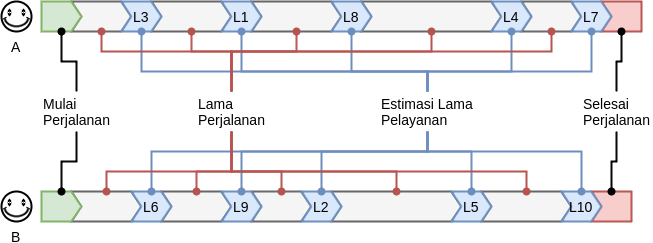
\includegraphics[width=\textwidth]{Resources/Images/illustration-timeline-mdvrp-timeservice-estimation}
		\caption{\textit{Timeline} Dengan Estimasi Waktu Pelayanan}
		\label{fig:illustration-timeline-mdvrp-timeservice-estimation}
	\end{subfigure}%
	
	\begin{subfigure}[t]{\textwidth}
		\centering
		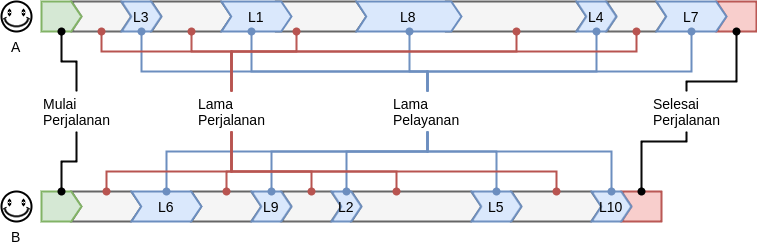
\includegraphics[width=\textwidth]{Resources/Images/illustration-timeline-mdvrp-timeservice-real}
		\caption{\textit{Timeline} Setelah Dikunjungi}
		\label{fig:illustration-timeline-mdvrp-timeservice-real}
	\end{subfigure}%
	\caption{\textit{Timeline} Sebelum dan Setelah Dikunjungi}
	\label{fig:illustration-timeline-mdvrp}
\end{figure}


Solusi yang ditawarkan agar rute yang dihasilkan memiliki total waktu pencacahan yang lebih \textit{equal} adalah dengan menggunakan mekanisme pencarian solusi secara bertahap (\autoref{fig:illustration-timeline-mdvrp-gradual-solution}). Setiap tahap pencarian solusi tidak dimaksudkan untuk mendapatkan rute lengkap secara keseluruhan, tetapi hanya digunakan untuk menentukan wilayah kerja yang akan dikunjungi berikutnya.


\begin{figure}[!]
	\centering
	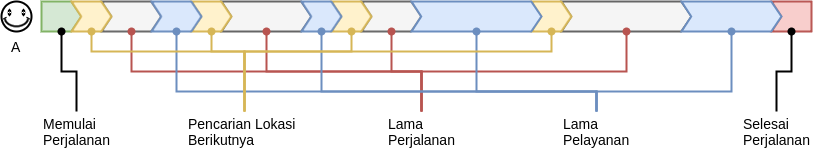
\includegraphics[width=\textwidth]{Resources/Images/illustration-timeline-mdvrp-gradual-solution}
	\caption{\textit{Timeline} Solusi Bertahap}
	\label{fig:illustration-timeline-mdvrp-gradual-solution}
\end{figure}


Agar `wilayah kerja berikutnya' yang dihasilkan lebih akurat, maka pencarian solusi harus dilakukan secara tersentral dengan melibatkan \textit{context} dari seluruh pencacah. Dalam sistem komputer tidak terdapat definisi \textit{context} yang tunggal. Sebagian besar peneliti sepakat bahwa \textit{context} adalah sesuatu yang harus dilakukan terkait interaksi pengguna dan sistem komputer \citep{chen_survey_2000}. \citep{schilit_context-aware_1994} dan  \citep{schmidt_there_1999}, misalnya, mendefinisikan \textit{context} sebagai pengetahuan tentang \textit{state} dari \textit{user} dan \textit{IT device}, termasuk lingkungan, situasi, dan lokasi. Sementara \citep{abowd_towards_1999} mendefinisikan \textit{context} sebagai segala informasi yang dapat digunakan untuk mengkarakterisasi kondisi dari suatu entitas.


Pencarian solusi secara tersentral membutuhkan mekanisme komunikasi antara \textit{client} (pencacah yang melakukan \textit{request} `wilayah kerja berikutnya') dan \textit{server} (pihak yang memproses \textit{request} dan mencari `wilayah kerja berikutnya'). Ada beragam opsi mekanisme komunikasi \textit{client-server} yang dapat digunakan, seperti \textit{Web service}, \textit{Request/Reply}, dan \textit{Publish/Subscribe} \citep{weise_solving_2009, sengoku_fast_1998, sarmenta_bayanihan_2002, muhl_large-scale_2002}. Mekanisme yang tepat diperlukan agar komunikasi antara \textit{client} dan \textit{server} dapat dilakukan dalam berbagai kondisi jaringan komunikasi.


Berdasarkan permasalahan diatas, penelitian ini dirancang untuk menciptakan sebuah sistem yang dapat digunakan dalam membuat rekomendasi lokasi pencacahan. Peneliti mengusulkan penggunaan mekanisme pencarian solusi secara bertahap dengan melibatkan \textit{context} dari pencacah dan mekanisme \textit{Publish/Subscribe}.


%-----------------------------------------------------------------------------%
\section{Rumusan Masalah}
%-----------------------------------------------------------------------------%
Berdasarkan latar belakang permasalahan yang telah diuraikan sebelumnya, maka dapat dirumuskan masalah dalam penelitian ini adalah bagaimana merancang sebuah sistem rekomendasi lokasi pencacahan sesuai dengan \textit{context} dari pencacah.


Adapun detail dari permasalahan yang akan dikaji adalah sebagai berikut:

\begin{itemize}
\item Bagaimana menentukan \textit{context} dari pencacah yang sesuai digunakan dalam kasus rekomendasi lokasi pencacahan?
\item Bagaimana menyusun algoritma pencarian rekomendasi lokasi dengan memanfaatkan \textit{context} dari pencacah?
\item Bagaimana menyusun mekanisme \textit{conflict resolution}, agar system tidak merekomendasikan lokasi yang sama pada dua atau lebih pencacah?
\item Apa mekanisme \textit{real-time} yang sesuai digunakan dalam berbagai kondisi jaringan komunikasi yang bervariasi?
\end{itemize}


%-----------------------------------------------------------------------------%
\section{Tujuan Penelitian}
%-----------------------------------------------------------------------------%
Berdasarkan rumusan masalah diatas, maka dapat ditentukan tujuan utama dari penelitian ini adalah untuk merancang sebuah arsitektur sistem rekomendasi lokasi pencacahan secara dinamis dan \textit{real-time}. 

Adapun tujuan khusus dari penelitian ini adalah:

\begin{itemize}
\item Menentukan \textit{context} yang sesuai dengan kasus rekomendasi lokasi pencacahan.
\item Menyusun algoritma rekomendasi lokasi sehingga sistem memberikan rekomendasi terbaik secara global.
\item Menyusun algoritma \textit{location conflict} sehingga sistem tidak memberikan duplikasi rekomendasi.
\item Menganalisis dan mengimplementasikan mekanisme komunikasi yang tepat digunakan pada sitem.
\end{itemize}


%-----------------------------------------------------------------------------%
\section{Batasan Masalah}
%-----------------------------------------------------------------------------%
Masalah dalam penelitian ini memiliki batasan sebagai berikut:

\begin{itemize}
\item Lokasi pencacahan yang menjadi rujukan adalah Blok Sensus (BS) yang dikeluarkan oleh Badan Pusat Statistik (BPS).
\item Penelitian tidak berfokus pada algoritma MDVRP, sehingga pengujian hanya dilakukan dengan membandingkan dengan salah satu algoritma MDVRP.
\end{itemize}


%-----------------------------------------------------------------------------%
\section{Manfaat dan Kontribusi}
%-----------------------------------------------------------------------------%
Hasil penelitian ini diharapkan dapat memberikan kontribusi kepada BPS khususnya, yaitu memudahkan \textit{subject matter} dalam melakukan alokasi petugas pencacahan. Ketepatan alokasi petugas memiliki implikasi pada meratanya beban setiap pencacah serta meratanya waktu penyelesaian pencacahan.


Selain itu, penelitian ini juga memberikan implikasi dalam bidang akademis, yaitu sistem tidak hanya dapat digunakan secara spesifik untuk kasus pengumpulan data, tetapi juga dapat digunakan pada kasus yang terkait dengan \textit{Vehicle Routing Problem}.


%-----------------------------------------------------------------------------%
\section{Sistematika Penulisan}
%-----------------------------------------------------------------------------%
Sistematika penulisan tesis ini terdiri atas enam bab dengan perincian sebagai berikut:


BAB I PENDAHULUAN. Pada bab ini dijelaskan fenomena dan masalah yang diangkat dalam penelitian ini. Selain itu dipaparkan pula mengenai rumusan masalah, tujuan penelitian, dan kontribusi penelitian.


BAB II STUDI LITERATUR. Bab ini menjelaskan landasan teori yang digunakan dalam penelitian, teknologi pendukung, serta penelitian terkait dengan penelitian yang dilakukan.


BAB III METODOLOGI PENELITIAN. Pada bagian ini dijelaskan metode penelitian yaitu alur dan langkah-langkah dalam melakukan penelitian.


BAB IV ANALISIS DAN PERANCANGAN. Bab ini memaparkan analisis terhadap permasalahan yang dihadapi, serta kriteria yang dibutuhkan pada algoritma yang dirancang. Dari analisis permasalahan, diuraikan pendekatan yang dibuat yang merupakan solusi atas permasalahan yang dikemukakan.


BAB V IMPLEMENTASI DAN PENGUJIAN. Proses dan hasil implementasi rancangan dijelaskan dalam bab ini. Proses pengujian diuraikan mulai dari skenario pengujian hingga hasil pengujian.


BAB VI KESIMPULAN DAN SARAN. Bab ini memaparkan kesimpulan yang diperoleh dari penelitian ini, serta saran untuk pihak terkait dan penelitian selanjutnya yang berkaitan dengan topik penelitian ini
